\documentclass[10pt]{beamer}

\usetheme{m}

\usepackage{booktabs}
\usepackage[scale=2]{ccicons}

\usepackage[T1]{fontenc}
\usepackage[brazil]{babel}
%\usepackage[latin1]{inputenc}

\usepackage{pgfplots}
\usepgfplotslibrary{dateplot}

\title{Aplicando o Arcabouço OpenTuner em Jogos Digitais}
\date{\today}
\author{Renan Teruo Carneiro e Vitor Cerqueira Santos\\
	Orientador: Prof. Dr. Alfredo Goldman\\
    Co-orientador: Pedro Bruel}
\institute{Instituto de Matemática e Estatística}
% \titlegraphic{\hfill\includegraphics[height=1.5cm]{logo/logo}}

\begin{document}

\maketitle

%\begin{frame}
%  \frametitle{Table of Contents}
%  \setbeamertemplate{section in toc}[sections numbered]
%  \tableofcontents[hideallsubsections]
%\end{frame}

\section{Introdução}

\begin{frame}[fragile]
	\frametitle{Otimização de Parâmetros}
	  \begin{itemize}
	  	\item Aplicação com várias configurações
	  	\item Problema: Encontrar melhor conjunto de configurações
	  	\item Autotuning é uma alternativa interessante
	  	\item Dentre os arcabouços de autotuning, OpenTuner se destaca
	  \end{itemize}
\end{frame}

\begin{frame}{OpenTuner}
	Arcabouço para Autotuning\\
	Apresenta diversas técnicas de busca\\
	'Exploitation' x 'Exploration'\\
	Infelizmente, ainda não oferece paralelismo na execução de testes
\end{frame}

\begin{frame}{OpenTuner}
	\begin{figure}
	\centering
	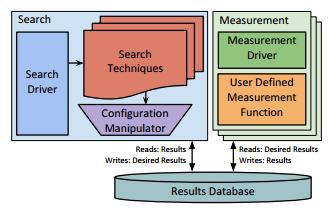
\includegraphics[width=1\linewidth]{OpenTuner}
	\caption{Estrutura do OpenTuner}
	\label{fig:OpenTuner}
	\end{figure}
\end{frame}
%
%\begin{frame}[fragile]
%  \frametitle{Ajuste Fino}
%	  Enter the Autotuning!
%	  \pause
%	  \begin{itemize}[<+- | alert@+>]
%	  	\item Automatiza esse processo:
%	  	\item   Chuta uma configuração
%	  	\item   Vê o resultado
%	  	\item   Chuta outra configuração baseado nisso
%	  \end{itemize} 
%  %TODO: Autotuning
%  
%\end{frame}
%
%\begin{frame}[fragile]
%	\frametitle{Ajuste Fino}
%	Imagem goes here? Suplanta slide anterior?
%\end{frame}
%
%\begin{frame}[fragile]
%	\frametitle{Ajuste Fino}
%	  \begin{itemize}[<+- | alert@+>]
%	  	\item Geralmente feito do zero
%	  	\item Pessoal tem que manjar não só o programa, mas também buscas
%	  	\item Demora pra fazer
%	  	\item \begin{verbatim}= (\end{verbatim}
%	\end{itemize}
%\end{frame}



%\begin{frame}[fragile]
%  \frametitle{OpenTuner}
%      OpenTuner!
%      \pause
%	  \begin{itemize}[<+- | alert@+>]
%		\item Já tem técnicas prontas
%		\item Só precisa passar o que rodar e os parâmetros
%		\item Não está pronto
%		\item KEDE PARALELISMO AAAAAAAAAAAAAA \begin{verbatim} >=(\end{verbatim}
%		
%	  \end{itemize}  
%\end{frame}

\section{Ideias}

\begin{frame}[fragile]
  \frametitle{Ideias}
	  \begin{itemize}
	  	\item Aplicações em jogos:
	  	\item Geradores de Mapa
	  	\item Inteligências Artificiais
	  	\item SaltyBet
	  	\item Builds de RPG e skilltrees
	  \end{itemize}
\end{frame}

\begin{frame}{Ideias}
	OpenTTD!
\end{frame}

\begin{frame}{OpenTTD}
	\begin{figure}
	\centering
	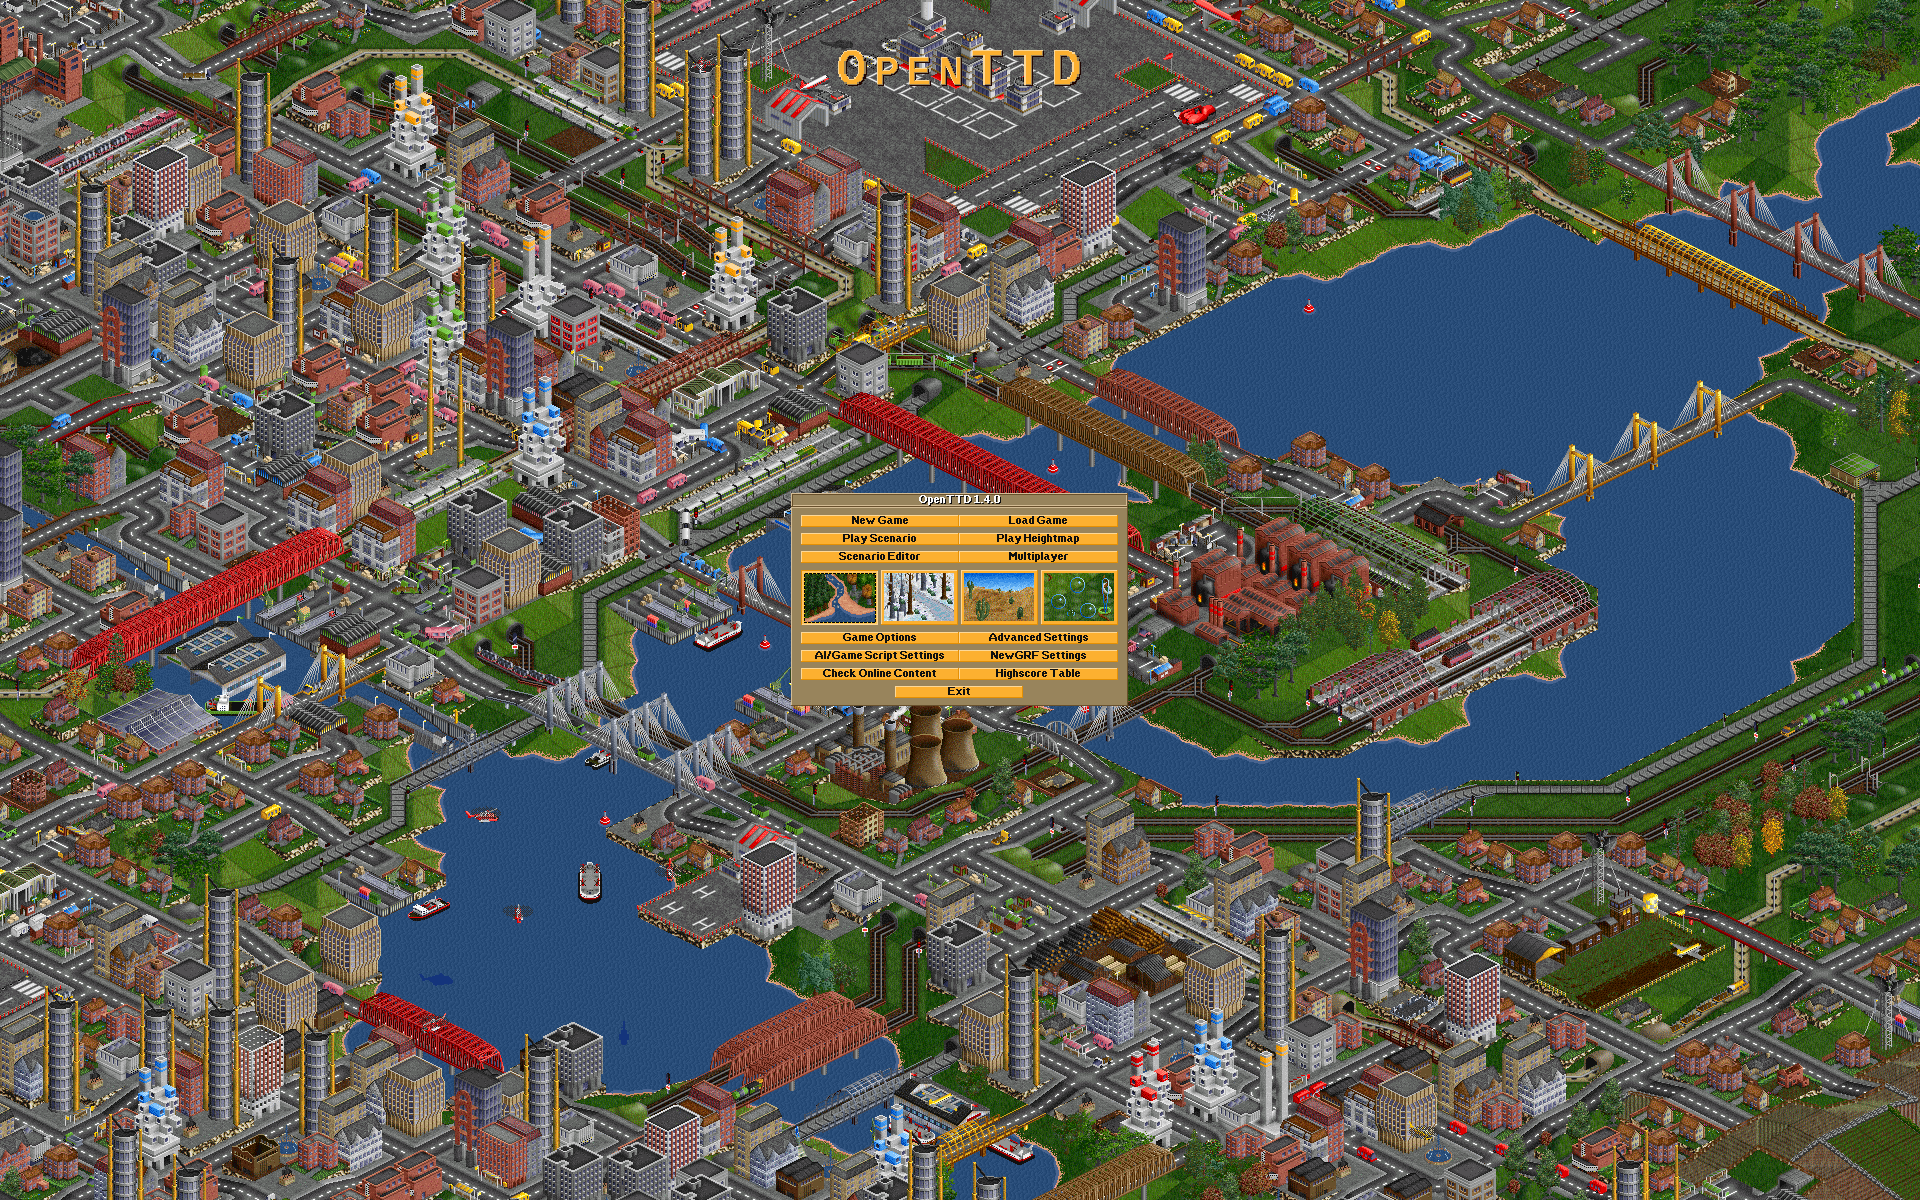
\includegraphics[width=1\linewidth]{OpenTTD}
	\caption{Tela inicial do OpenTTD}
	\label{fig:OpenTTD}
	\end{figure}
\end{frame}

\begin{frame}{OpenTTD}	
	\begin{itemize}	
		\item Simulador de gerência de uma empresa de transportes
		\item Projeto Open Source
		\item Possui suporte para IAs
		\item Um dos aspectos mais detalhados do jogo é a malha de trens
	\end{itemize}
\end{frame}

\section{Experimentos}
\begin{frame}{Experimentos}
	Verificar os resultados de alterar os custos do \textit{pathfinder} de uma IA.\\
	Para isso, escolhemos a IA ChooChoo, que é focada em trens.
\end{frame}

\begin{frame}{Experimentos}
	\begin{figure}
\centering
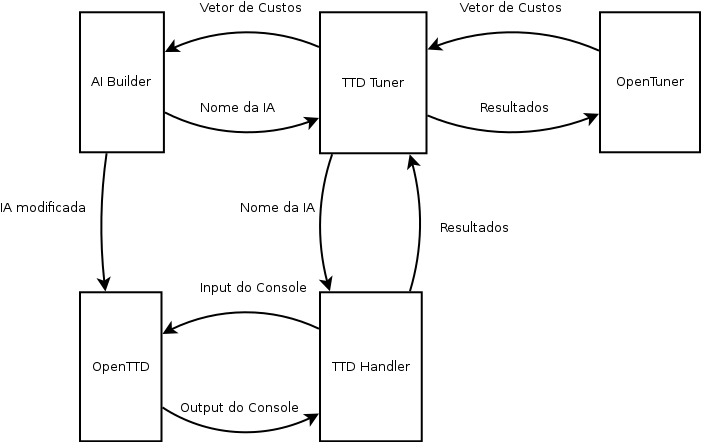
\includegraphics[width=1\linewidth]{Diagrama1}
\caption{Estrutura do tuner}
\label{fig:Diagrama1}
\end{figure}

\end{frame}
	
\begin{frame}{Experimentos}
	\begin{itemize}
	\item Diversas adaptações feitas para o funcionamento do OpenTTD junto com o OpenTuner \\
%	Builder <-> Tuner <-> Handler <-> OpenTTD <-> TRENS!!!!\pause\\
	\item OpenTTD compilado para funcionar em uma velocidade muito maior que a normal\\
	\item Pode medir valor da empresa, dinheiro em caixa ou lucro no último quartil\\
	\item Mede ao final de N anos, configurável\\
	\item Suporta iterações de 1 $\leq$ N $\leq$ 14 IAs, tirando média dos valores obtidos\\
	\item Foram feitos testes de 10 e 30 anos para lucro e caixa, e 10 e 50 para valor da empresa, com 6 ou 8 IAs por teste\\
	\item Demora para gerar resultados -> Utilizando máquinas não-dedicadas\\
	\item Certa instabilidade
	\end{itemize}
\end{frame}

\section{Resultados e Conclusões}

\begin{frame}{Resultados e conclusões}
	\begin{figure}
		\centering
		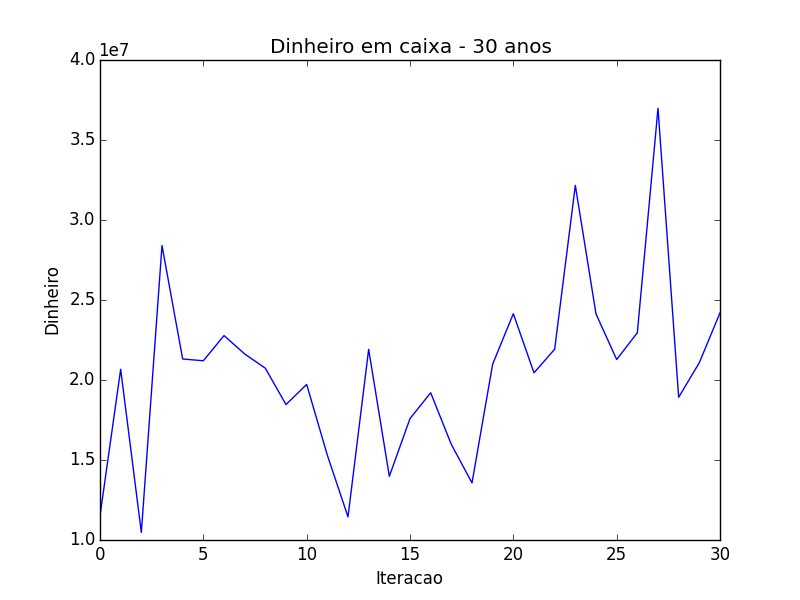
\includegraphics[width=1\linewidth]{money-30yrs}
		\caption{Resultados dos testes para 30 anos}
		\label{fig:money-30yrs}
	\end{figure}
	
\end{frame}

\begin{frame}{Resultados e conclusões}
	\begin{figure}
		\centering
		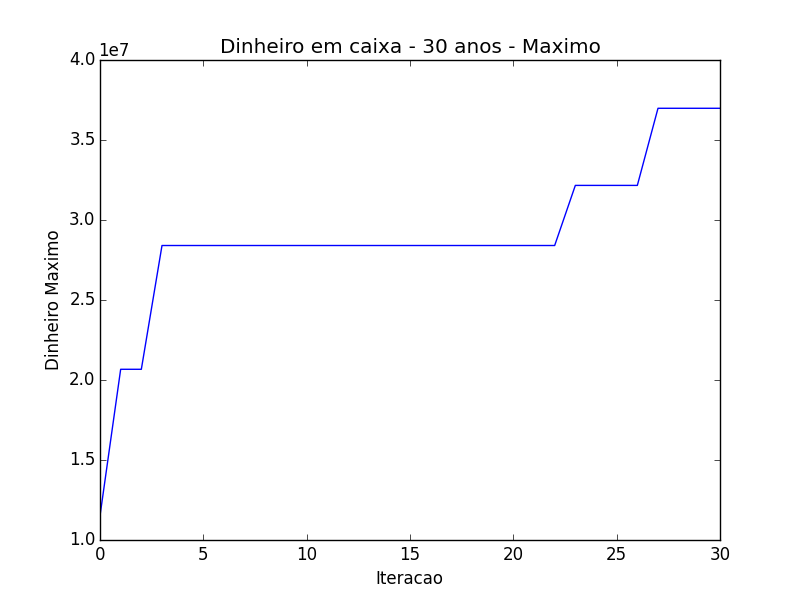
\includegraphics[width=1\linewidth]{money-30yrs-best}
		\caption{Resultados dos testes para 30 anos}
		\label{fig:money-30yrs-best}
	\end{figure}
	
\end{frame}

\begin{frame}{Resultados e conclusões}
	\begin{figure}
		\centering
		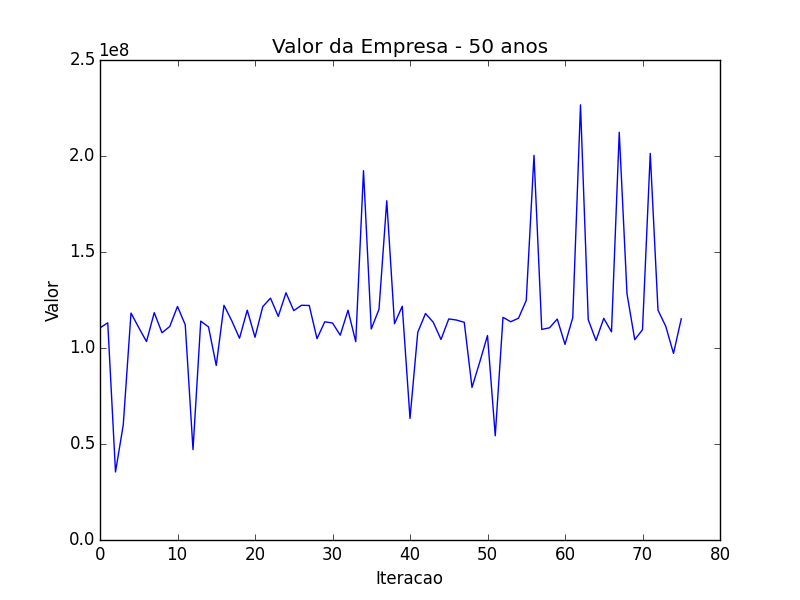
\includegraphics[width=1\linewidth]{value-50yrs}
		\caption{Resultados dos testes para 50 anos}
		\label{fig:value-50yrs}
	\end{figure}
	
\end{frame}

\begin{frame}{Resultados e conclusões}
	\begin{figure}
		\centering
		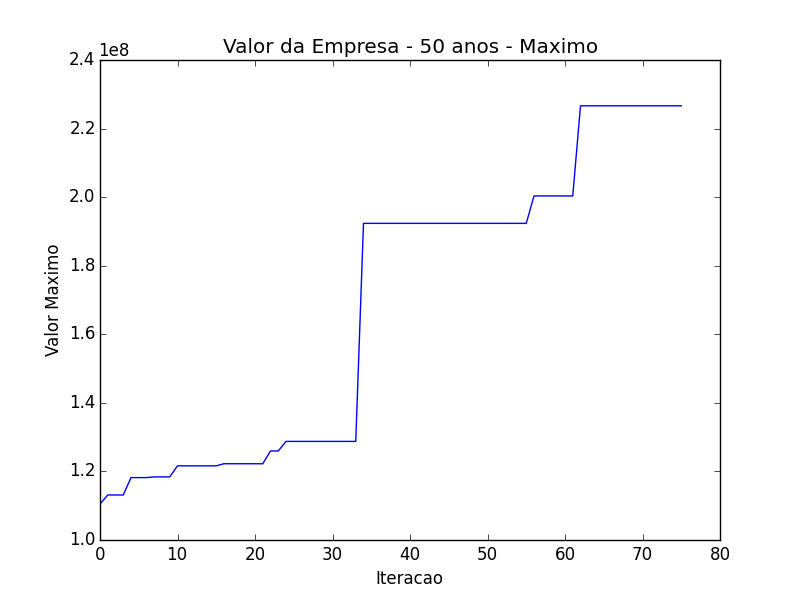
\includegraphics[width=1\linewidth]{value-50yrs-best}
		\caption{Resultados dos testes para 50 anos}
		\label{fig:value-50yrs-best}
	\end{figure}
	
\end{frame}

\begin{frame}{Resultados e conclusões}
	\begin{figure}
		\centering
		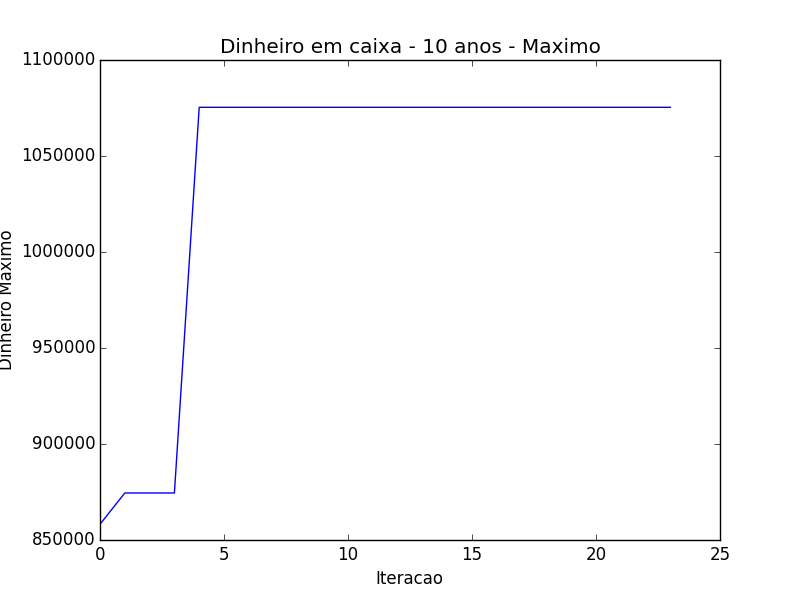
\includegraphics[width=1\linewidth]{money-10yrs-best}
		\caption{Resultados dos testes para 10 anos}
		\label{fig:money-10yrs-best}
	\end{figure}
	
\end{frame}

\begin{frame}{Resultados e Conclusões}
	\begin{itemize}
	\item Funciona!  De certa forma\\
	\item OpenTuner conseguiu resultados sem saber intrinsecamente como o programa funciona \\
	\item Custos de pathfinder tem resultados significativos em um aspecto maior do jogo\\
	\item OpenTTD não foi feito pra ser automatizado, então usar o OpenTuner necessitou algumas adaptações\\
	\item Talvez seja mais útil se um jogo for desenvolvido desde o começo com isso em mente
	\end{itemize}
\end{frame}

\begin{frame}{Considerações finais}
	Obrigado! Dúvidas?\\
	Referências/Links:\\
	\begin{itemize}
		\item Ansel, Jason, et al. "Opentuner: An extensible framework for program autotuning." Proceedings of the 23rd international conference on Parallel architectures and compilation. ACM, 2014.
		\item OpenTTD: https://www.openttd.org/en/, Novembro 2015
		\item GitHub do projeto: https://github.com/imano-ob/opentunerstuff-openttd
	\end{itemize}
\end{frame}

\end{document}
